\documentclass[twoside]{book}

% Packages required by doxygen
\usepackage{calc}
\usepackage{doxygen}
\usepackage{graphicx}
\usepackage[utf8]{inputenc}
\usepackage{makeidx}
\usepackage{multicol}
\usepackage{multirow}
\usepackage{textcomp}
\usepackage[table]{xcolor}

% Font selection
\usepackage[T1]{fontenc}
\usepackage{mathptmx}
\usepackage[scaled=.90]{helvet}
\usepackage{courier}
\usepackage{amssymb}
\usepackage{sectsty}
\renewcommand{\familydefault}{\sfdefault}
\allsectionsfont{%
  \fontseries{bc}\selectfont%
  \color{darkgray}%
}
\renewcommand{\DoxyLabelFont}{%
  \fontseries{bc}\selectfont%
  \color{darkgray}%
}

% Page & text layout
\usepackage{geometry}
\geometry{%
  a4paper,%
  top=2.5cm,%
  bottom=2.5cm,%
  left=2.5cm,%
  right=2.5cm%
}
\tolerance=750
\hfuzz=15pt
\hbadness=750
\setlength{\emergencystretch}{15pt}
\setlength{\parindent}{0cm}
\setlength{\parskip}{0.2cm}
\makeatletter
\renewcommand{\paragraph}{%
  \@startsection{paragraph}{4}{0ex}{-1.0ex}{1.0ex}{%
    \normalfont\normalsize\bfseries\SS@parafont%
  }%
}
\renewcommand{\subparagraph}{%
  \@startsection{subparagraph}{5}{0ex}{-1.0ex}{1.0ex}{%
    \normalfont\normalsize\bfseries\SS@subparafont%
  }%
}
\makeatother

% Headers & footers
\usepackage{fancyhdr}
\pagestyle{fancyplain}
\fancyhead[LE]{\fancyplain{}{\bfseries\thepage}}
\fancyhead[CE]{\fancyplain{}{}}
\fancyhead[RE]{\fancyplain{}{\bfseries\leftmark}}
\fancyhead[LO]{\fancyplain{}{\bfseries\rightmark}}
\fancyhead[CO]{\fancyplain{}{}}
\fancyhead[RO]{\fancyplain{}{\bfseries\thepage}}
\fancyfoot[LE]{\fancyplain{}{}}
\fancyfoot[CE]{\fancyplain{}{}}
\fancyfoot[RE]{\fancyplain{}{\bfseries\scriptsize Generated on Fri Jan 23 2015 01\-:09\-:19 for My Project by Doxygen }}
\fancyfoot[LO]{\fancyplain{}{\bfseries\scriptsize Generated on Fri Jan 23 2015 01\-:09\-:19 for My Project by Doxygen }}
\fancyfoot[CO]{\fancyplain{}{}}
\fancyfoot[RO]{\fancyplain{}{}}
\renewcommand{\footrulewidth}{0.4pt}
\renewcommand{\chaptermark}[1]{%
  \markboth{#1}{}%
}
\renewcommand{\sectionmark}[1]{%
  \markright{\thesection\ #1}%
}

% Indices & bibliography
\usepackage{natbib}
\usepackage[titles]{tocloft}
\setcounter{tocdepth}{3}
\setcounter{secnumdepth}{5}
\makeindex

% Hyperlinks (required, but should be loaded last)
\usepackage{ifpdf}
\ifpdf
  \usepackage[pdftex,pagebackref=true]{hyperref}
\else
  \usepackage[ps2pdf,pagebackref=true]{hyperref}
\fi
\hypersetup{%
  colorlinks=true,%
  linkcolor=blue,%
  citecolor=blue,%
  unicode%
}

% Custom commands
\newcommand{\clearemptydoublepage}{%
  \newpage{\pagestyle{empty}\cleardoublepage}%
}


%===== C O N T E N T S =====

\begin{document}

% Titlepage & ToC
\hypersetup{pageanchor=false}
\pagenumbering{roman}
\begin{titlepage}
\vspace*{7cm}
\begin{center}%
{\Large My Project }\\
\vspace*{1cm}
{\large Generated by Doxygen 1.8.6}\\
\vspace*{0.5cm}
{\small Fri Jan 23 2015 01:09:19}\\
\end{center}
\end{titlepage}
\clearemptydoublepage
\tableofcontents
\clearemptydoublepage
\pagenumbering{arabic}
\hypersetup{pageanchor=true}

%--- Begin generated contents ---
\chapter{Hierarchical Index}
\section{Class Hierarchy}
This inheritance list is sorted roughly, but not completely, alphabetically\-:\begin{DoxyCompactList}
\item \contentsline{section}{Figura\-:\-:Figura}{\pageref{classFigura_1_1Figura}}{}
\begin{DoxyCompactList}
\item \contentsline{section}{Figura\-:\-:Circulo}{\pageref{classFigura_1_1Circulo}}{}
\item \contentsline{section}{Figura\-:\-:Cuadrado}{\pageref{classFigura_1_1Cuadrado}}{}
\end{DoxyCompactList}
\end{DoxyCompactList}

\chapter{Class Index}
\section{Class List}
Here are the classes, structs, unions and interfaces with brief descriptions\-:\begin{DoxyCompactList}
\item\contentsline{section}{\hyperlink{classFigura_1_1Circulo}{Figura\-::\-Circulo} }{\pageref{classFigura_1_1Circulo}}{}
\item\contentsline{section}{\hyperlink{classFigura_1_1Cuadrado}{Figura\-::\-Cuadrado} }{\pageref{classFigura_1_1Cuadrado}}{}
\item\contentsline{section}{\hyperlink{classFigura_1_1Figura}{Figura\-::\-Figura} }{\pageref{classFigura_1_1Figura}}{}
\end{DoxyCompactList}

\chapter{File Index}
\section{File List}
Here is a list of all documented files with brief descriptions\-:\begin{DoxyCompactList}
\item\contentsline{section}{\hyperlink{namespace_8cc}{namespace.\-cc} \\*Fichero con algunas funciones }{\pageref{namespace_8cc}}{}
\item\contentsline{section}{{\bfseries namespace.\-h} }{\pageref{namespace_8h}}{}
\end{DoxyCompactList}

\chapter{Class Documentation}
\hypertarget{classFigura_1_1Circulo}{\section{Figura\-:\-:Circulo Class Reference}
\label{classFigura_1_1Circulo}\index{Figura\-::\-Circulo@{Figura\-::\-Circulo}}
}
Inheritance diagram for Figura\-:\-:Circulo\-:\begin{figure}[H]
\begin{center}
\leavevmode
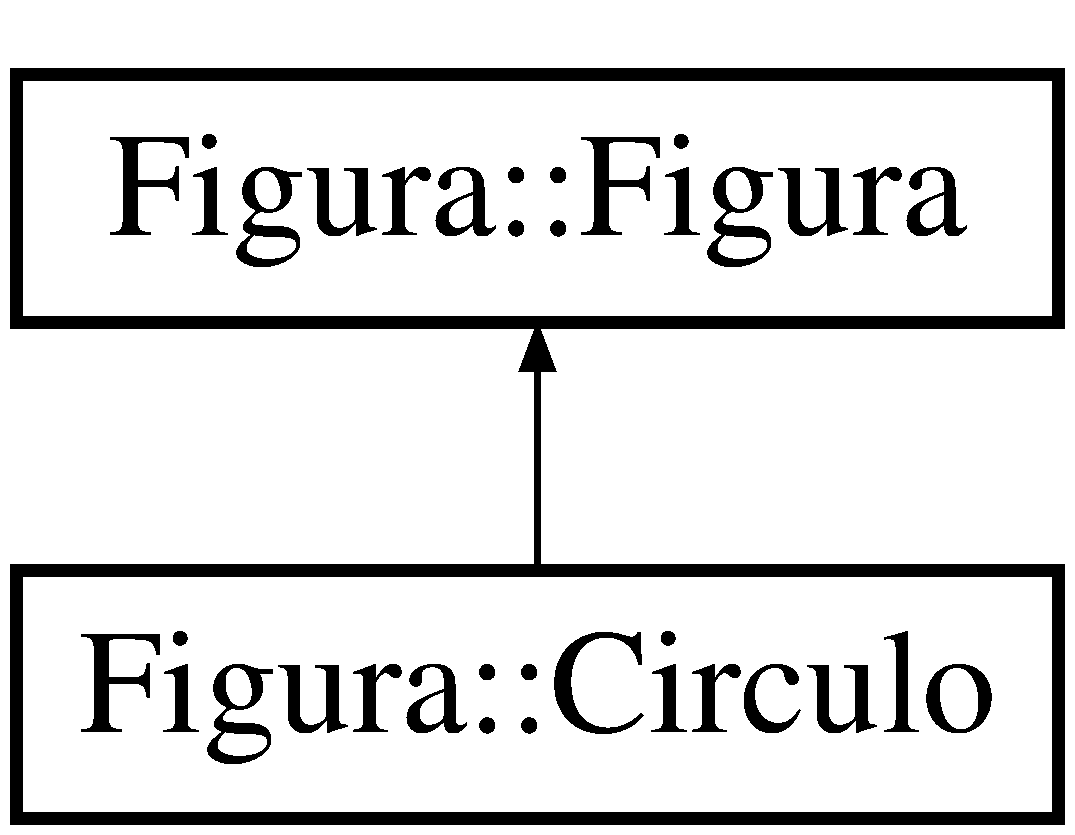
\includegraphics[height=2.000000cm]{classFigura_1_1Circulo}
\end{center}
\end{figure}
\subsection*{Public Member Functions}
\begin{DoxyCompactItemize}
\item 
\hypertarget{classFigura_1_1Circulo_ae53a2338b51e222030eec73a59dc9b8a}{{\bfseries Circulo} (double radio, string n)}\label{classFigura_1_1Circulo_ae53a2338b51e222030eec73a59dc9b8a}

\item 
\hypertarget{classFigura_1_1Circulo_a1e4475d8d704ac3133836ba3653855c0}{virtual double {\bfseries area} ()}\label{classFigura_1_1Circulo_a1e4475d8d704ac3133836ba3653855c0}

\item 
\hypertarget{classFigura_1_1Circulo_a6d1806b05698060c90c92e0679b76f1c}{virtual double {\bfseries perimetro} ()}\label{classFigura_1_1Circulo_a6d1806b05698060c90c92e0679b76f1c}

\end{DoxyCompactItemize}


The documentation for this class was generated from the following files\-:\begin{DoxyCompactItemize}
\item 
namespace.\-h\item 
main.\-cc\item 
\hyperlink{namespace_8cc}{namespace.\-cc}\end{DoxyCompactItemize}

\hypertarget{classFigura_1_1Cuadrado}{\section{Figura\-:\-:Cuadrado Class Reference}
\label{classFigura_1_1Cuadrado}\index{Figura\-::\-Cuadrado@{Figura\-::\-Cuadrado}}
}
Inheritance diagram for Figura\-:\-:Cuadrado\-:\begin{figure}[H]
\begin{center}
\leavevmode
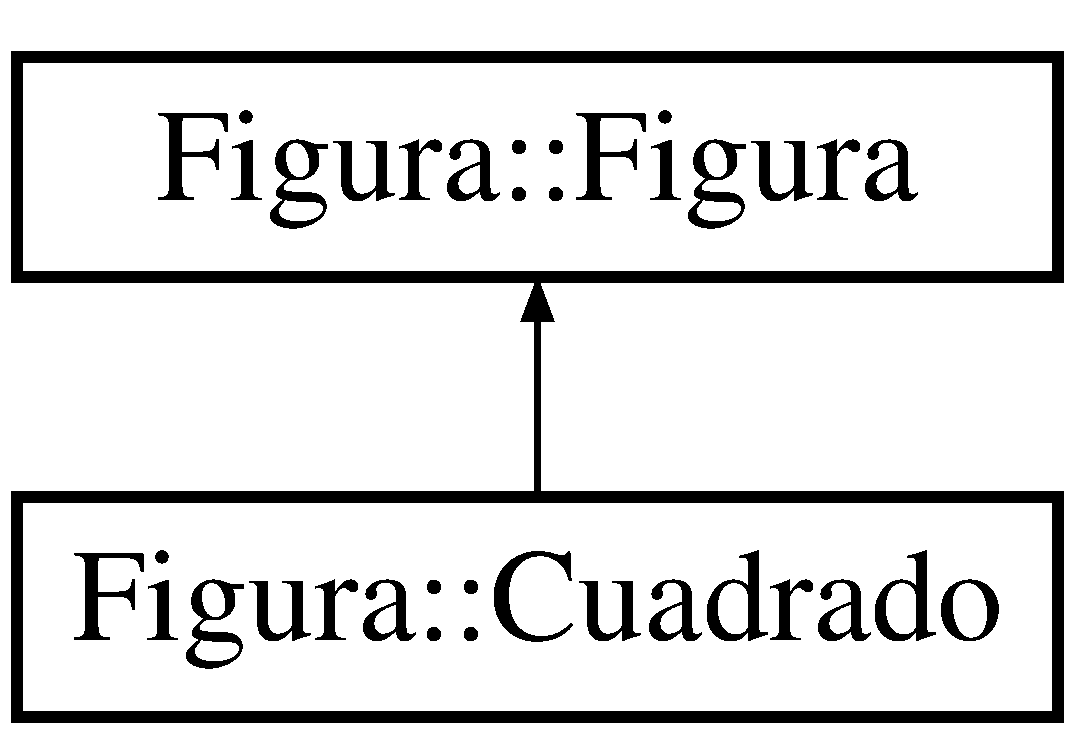
\includegraphics[height=2.000000cm]{classFigura_1_1Cuadrado}
\end{center}
\end{figure}
\subsection*{Public Member Functions}
\begin{DoxyCompactItemize}
\item 
\hypertarget{classFigura_1_1Cuadrado_a72df40724ac3aee7cf80d646822be195}{{\bfseries Cuadrado} (double lado, string n)}\label{classFigura_1_1Cuadrado_a72df40724ac3aee7cf80d646822be195}

\item 
virtual double \hyperlink{classFigura_1_1Cuadrado_a35188b1bf04298411e470fe92a42222b}{area} ()
\begin{DoxyCompactList}\small\item\em Devuelve el area del cuadrado. \end{DoxyCompactList}\item 
\hypertarget{classFigura_1_1Cuadrado_aeeff15d5db282739ddf4ff86658a1ed0}{virtual double {\bfseries perimetro} ()}\label{classFigura_1_1Cuadrado_aeeff15d5db282739ddf4ff86658a1ed0}

\end{DoxyCompactItemize}


\subsection{Member Function Documentation}
\hypertarget{classFigura_1_1Cuadrado_a35188b1bf04298411e470fe92a42222b}{\index{Figura\-::\-Cuadrado@{Figura\-::\-Cuadrado}!area@{area}}
\index{area@{area}!Figura::Cuadrado@{Figura\-::\-Cuadrado}}
\subsubsection[{area}]{\setlength{\rightskip}{0pt plus 5cm}double Figura\-::\-Cuadrado\-::area (
\begin{DoxyParamCaption}
{}
\end{DoxyParamCaption}
)\hspace{0.3cm}{\ttfamily [virtual]}}}\label{classFigura_1_1Cuadrado_a35188b1bf04298411e470fe92a42222b}


Devuelve el area del cuadrado. 


\begin{DoxyParams}{Parameters}
{\em ninguno} & \\
\hline
{\em puesnah} & \\
\hline
\end{DoxyParams}
\begin{DoxyReturn}{Returns}
lado$\ast$lado 
\end{DoxyReturn}


Implements \hyperlink{classFigura_1_1Figura}{Figura\-::\-Figura}.



The documentation for this class was generated from the following files\-:\begin{DoxyCompactItemize}
\item 
namespace.\-h\item 
\hyperlink{namespace_8cc}{namespace.\-cc}\end{DoxyCompactItemize}

\hypertarget{classFigura_1_1Figura}{\section{Figura\-:\-:Figura Class Reference}
\label{classFigura_1_1Figura}\index{Figura\-::\-Figura@{Figura\-::\-Figura}}
}
Inheritance diagram for Figura\-:\-:Figura\-:\begin{figure}[H]
\begin{center}
\leavevmode
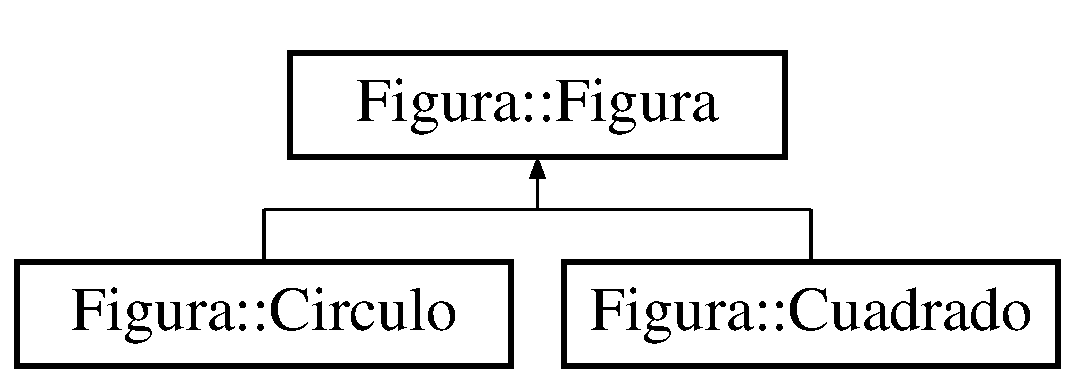
\includegraphics[height=2.000000cm]{classFigura_1_1Figura}
\end{center}
\end{figure}
\subsection*{Public Member Functions}
\begin{DoxyCompactItemize}
\item 
\hypertarget{classFigura_1_1Figura_a5fca1cc004e13574d31f7a5f3afd4039}{{\bfseries Figura} (string n)}\label{classFigura_1_1Figura_a5fca1cc004e13574d31f7a5f3afd4039}

\item 
\hypertarget{classFigura_1_1Figura_add6081ce2446a4919b106313546316ac}{string {\bfseries nombre} ()}\label{classFigura_1_1Figura_add6081ce2446a4919b106313546316ac}

\item 
\hypertarget{classFigura_1_1Figura_a72ce7658ac247e7ce85601df372129a9}{virtual double {\bfseries area} ()=0}\label{classFigura_1_1Figura_a72ce7658ac247e7ce85601df372129a9}

\item 
\hypertarget{classFigura_1_1Figura_a31f599da6f2d170b50121bd3a6bc4898}{virtual double {\bfseries perimetro} ()=0}\label{classFigura_1_1Figura_a31f599da6f2d170b50121bd3a6bc4898}

\end{DoxyCompactItemize}


The documentation for this class was generated from the following file\-:\begin{DoxyCompactItemize}
\item 
namespace.\-h\end{DoxyCompactItemize}

\chapter{File Documentation}
\hypertarget{namespace_8cc}{\section{namespace.\-cc File Reference}
\label{namespace_8cc}\index{namespace.\-cc@{namespace.\-cc}}
}


Fichero con algunas funciones.  


{\ttfamily \#include \char`\"{}namespace.\-h\char`\"{}}\\*
{\ttfamily \#include $<$string$>$}\\*


\subsection{Detailed Description}
Fichero con algunas funciones. \begin{DoxyAuthor}{Author}
Ruben 
\end{DoxyAuthor}
\begin{DoxyDate}{Date}
hoy 
\end{DoxyDate}

%--- End generated contents ---

% Index
\newpage
\phantomsection
\addcontentsline{toc}{chapter}{Index}
\printindex

\end{document}
